\documentclass[aspectratio=169]{beamer}

\usepackage{iftex}
\providecommand{\dunenoirsetupfonts}{}
\newcommand{\DuneNoirLocalFontPath}{fonts}

\newcommand{\DuneNoirMonoFallback}{%
  \IfFontExistsTF{JetBrainsMono Nerd Font Propo}{
    \setmonofont{JetBrainsMono Nerd Font Propo}[Scale=0.92]
  }{
    \IfFontExistsTF{JetBrainsMono Nerd Font}{
      \setmonofont{JetBrainsMono Nerd Font}[Scale=0.92]
    }{
      \setmonofont{Courier New}[Scale=0.92]
    }
  }
}

\newcommand{\DuneNoirSansFallback}{%
  \IfFontExistsTF{IBM Plex Sans}{
    \setsansfont{IBM Plex Sans}
    \setmainfont{IBM Plex Sans}
  }{
    \IfFontExistsTF{Helvetica Neue}{
      \setsansfont{Helvetica Neue}
      \setmainfont{Helvetica Neue}
    }{
      \setsansfont{Arial}
      \setmainfont{Arial}
    }
  }
}

\newcommand{\DuneNoirUseHelvetica}{%
  \renewcommand{\dunenoirsetupfonts}{%
    \IfFontExistsTF{Helvetica Neue}{
      \setsansfont{Helvetica Neue}
      \setmainfont{Helvetica Neue}
    }{
      \IfFontExistsTF{Helvetica}{
        \setsansfont{Helvetica}
        \setmainfont{Helvetica}
      }{
        \DuneNoirSansFallback
      }
    }
    \DuneNoirMonoFallback
  }%
}

\newcommand{\DuneNoirUseOpenSans}{%
  \renewcommand{\dunenoirsetupfonts}{%
    \IfFileExists{\DuneNoirLocalFontPath/OpenSans.ttf}{
      \setsansfont{Open Sans Custom}[
        Path=\DuneNoirLocalFontPath/,
        UprightFont={OpenSans.ttf},
        ItalicFont={OpenSans-Italic.ttf},
        BoldFont={OpenSans.ttf},
        BoldItalicFont={OpenSans-Italic.ttf},
        BoldFeatures={FakeBold=1.45},
        BoldItalicFeatures={FakeBold=1.45}
      ]
      \setmainfont{Open Sans Custom}[
        Path=\DuneNoirLocalFontPath/,
        UprightFont={OpenSans.ttf},
        ItalicFont={OpenSans-Italic.ttf},
        BoldFont={OpenSans.ttf},
        BoldItalicFont={OpenSans-Italic.ttf},
        BoldFeatures={FakeBold=1.45},
        BoldItalicFeatures={FakeBold=1.45}
      ]
    }{
      \DuneNoirSansFallback
    }
    \DuneNoirMonoFallback
  }%
}

\newcommand{\DuneNoirUseDosis}{%
  \renewcommand{\dunenoirsetupfonts}{%
    \IfFileExists{\DuneNoirLocalFontPath/Dosis.ttf}{
      \setsansfont{Dosis Custom}[
        Path=\DuneNoirLocalFontPath/,
        UprightFont={Dosis.ttf},
        ItalicFont={Dosis.ttf},
        BoldFont={Dosis.ttf},
        BoldItalicFont={Dosis.ttf},
        ItalicFeatures={FakeSlant=0.16},
        BoldFeatures={FakeBold=1.6},
        BoldItalicFeatures={FakeBold=1.6,FakeSlant=0.16}
      ]
      \setmainfont{Dosis Custom}[
        Path=\DuneNoirLocalFontPath/,
        UprightFont={Dosis.ttf},
        ItalicFont={Dosis.ttf},
        BoldFont={Dosis.ttf},
        BoldItalicFont={Dosis.ttf},
        ItalicFeatures={FakeSlant=0.16},
        BoldFeatures={FakeBold=1.6},
        BoldItalicFeatures={FakeBold=1.6,FakeSlant=0.16}
      ]
    }{
      \DuneNoirSansFallback
    }
    \DuneNoirMonoFallback
  }%
}

\newcommand{\DuneNoirUseKoHo}{%
  \renewcommand{\dunenoirsetupfonts}{%
    \IfFileExists{\DuneNoirLocalFontPath/KoHo-Regular.ttf}{
      \setsansfont{KoHo Custom}[
        Path=\DuneNoirLocalFontPath/,
        UprightFont={KoHo-Regular.ttf},
        BoldFont={KoHo-Bold.ttf},
        ItalicFont={KoHo-Italic.ttf},
        BoldItalicFont={KoHo-BoldItalic.ttf}
      ]
      \setmainfont{KoHo Custom}[
        Path=\DuneNoirLocalFontPath/,
        UprightFont={KoHo-Regular.ttf},
        BoldFont={KoHo-Bold.ttf},
        ItalicFont={KoHo-Italic.ttf},
        BoldItalicFont={KoHo-BoldItalic.ttf}
      ]
    }{
      \DuneNoirSansFallback
    }
    \DuneNoirMonoFallback
  }%
}

\DuneNoirUseHelvetica
\usetheme{DUNENoir}
\beamertemplatenavigationsymbolsempty

\ifPDFTeX
  \usepackage[T1]{fontenc}
  \usepackage[utf8]{inputenc}
\fi
\usepackage{graphicx}
\usepackage{amsmath}
\usepackage{array}
\usepackage{booktabs}
\usepackage{hyperref}
\usepackage{siunitx}
\usepackage{tabularx}
\usepackage[dvipsnames]{xcolor}

\title[DAPHNE to TP]{From DAPHNE Descriptors to DUNE-DAQ Trigger Primitives}
\subtitle{Non-beam and low-energy PDS signatures}
\author{Manuel Arroyave}
\date{April 20, 2026}
\newcommand{\mydate}{April 20, 2026}
\newcommand{\sectioncard}[2]{%
  \begin{frame}[plain]
    \begin{tikzpicture}[remember picture,overlay]
      \fill[noirpanelalt] (current page.south west) rectangle (current page.north east);
      \fill[duneorange] ($(current page.north west)+(0.9,-0.9)$) rectangle ++(1.8,0.08);
      \fill[noircyan] ($(current page.south east)+(-2.8,0.9)$) rectangle ++(1.8,0.08);
      \draw[noirline, line width=0.8pt] ($(current page.south west)+(0.9,1.1)$) -- ($(current page.south east)+(-0.9,1.1)$);
    \end{tikzpicture}
    \vspace*{0.21\paperheight}
    {\color{noirmuted}\small\bfseries SECTION\par}
    \vspace{3mm}
    {\color{white}\bfseries\fontsize{29}{32}\selectfont #1\par}
    \vspace{4mm}
    {\color{noirmuted}\fontsize{13}{16}\selectfont #2\par}
  \end{frame}
}

\begin{document}

{
\setbeamertemplate{headline}{}
\setbeamertemplate{footline}{}
\begin{frame}[plain,noframenumbering]
  \titlepage
\end{frame}
}

\sectioncard{Physics Context}{What kind of light signatures matter, and what one board can or cannot decide}

\begin{frame}{One-Slide Thesis}
\small
\begin{block}{Physics signatures}
For this trigger discussion, the relevant PDS cases are:
\begin{itemize}
  \item prompt local light
  \item possible delayed local activity
  \item detector-wide low-light rate excess
\end{itemize}
\end{block}

\begin{alertblock}{Architecture consequence}
One DAPHNE board only measures \alert{channel-local} timing and pulse-shape observables. Firmware should export those descriptors so DAQ can build \texttt{TriggerPrimitive} objects and make detector-level decisions downstream.
\end{alertblock}
\end{frame}

\begin{frame}{Three Layers We Must Not Mix}
\small
\begin{columns}[T,onlytextwidth]
\column{0.32\linewidth}
\begin{block}{Physics in LAr}
Expected footprint:
\begin{itemize}
  \item local flash
  \item delayed local activity
  \item sparse detector-wide burst
\end{itemize}
\end{block}

\column{0.32\linewidth}
\begin{block}{Board firmware}
What one board measures:
\begin{itemize}
  \item timestamp
  \item width, peak, integral
  \item peak count, quality bits
\end{itemize}
\end{block}

\column{0.32\linewidth}
\begin{block}{DAQ trigger}
What the detector decides:
\begin{itemize}
  \item TP, TA, TC, TD
  \item clustering across boards
  \item long time-window logic
\end{itemize}
\end{block}
\end{columns}

\vspace{1mm}
\begin{alertblock}{Working rule}
\centering
\textbf{signature in LAr} \(\rightarrow\) \textbf{descriptor in firmware} \(\rightarrow\) \textbf{trigger object in DAQ}
\end{alertblock}
\end{frame}

\begin{frame}{What The DUNE Literature Supports}
\small
\begin{block}{Claim 1: PDS is not only for beam timing}
DUNE PDS is explicitly relevant for non-beam triggering, \textit{t0}, supernova sensitivity, and nucleon-decay-motivated searches.
\end{block}

\begin{block}{Claim 2: Supernova is a rate problem}
The useful signature is not one bright flash; it is a detector-wide excess of many low-light interactions over \(\mathrm{ms}\) to \(\mathrm{s}\) windows.
\end{block}

\begin{block}{Claim 3: Very-low-energy light is noise-limited}
Standalone optical triggering near threshold remains difficult; baseline stability and noise rejection are still central.
\end{block}
\end{frame}

\sectioncard{Firmware to DAQ}{What DAPHNE exports, what DAQ already defines, and what we need to validate}

\begin{frame}{What One DAPHNE Board Can Export}
\small
\begin{columns}[t]
\column{0.49\linewidth}
\begin{block}{Timing and trigger context}
\texttt{trigger\_timestamp}, \texttt{baseline}, filtered samples, and \texttt{trigger\_pulse}.
\end{block}

\column{0.49\linewidth}
\begin{block}{Pulse descriptors}
\texttt{time\_start}, \texttt{time\_peak}, \texttt{time\_over\_baseline}, \texttt{adc\_peak}, \texttt{adc\_integral}, \texttt{number\_peaks}, and quality bits.
\end{block}
\end{columns}

\vspace{0.5mm}
\begin{alertblock}{Important limitation}
The public boundary still exports \texttt{TRIGGER\_DESCRIPTOR\_NULL}; the TP-facing export contract is not the finished firmware boundary yet.
\end{alertblock}
\end{frame}

\begin{frame}{Descriptors to DAQ Trigger Primitives}
\small
\begin{block}{Direct mappings}
\renewcommand{\arraystretch}{1.06}
\begin{tabularx}{\linewidth}{>{\ttfamily\raggedright\arraybackslash}X c >{\ttfamily\raggedright\arraybackslash}X}
time\_peak & \(\rightarrow\) & samples\_to\_peak \\
time\_over\_baseline & \(\rightarrow\) & samples\_over\_threshold \\
adc\_peak & \(\rightarrow\) & adc\_peak \\
adc\_integral & \(\rightarrow\) & adc\_integral \\
\multicolumn{3}{@{}l@{}}{waveform timestamp + sample offset \(\rightarrow\) TP start timestamp}
\end{tabularx}
\end{block}

\begin{alertblock}{Reading}
Firmware fills the local pulse quantities; DAQ instantiates the common \texttt{TriggerPrimitive} object.
\end{alertblock}
\end{frame}

\begin{frame}{What The DAQ Contract Already Defines}
\small
\begin{block}{Already defined downstream}
\begin{itemize}
  \item TP bit widths and quality semantics
  \item channel and detector mapping path via \texttt{detchannelmaps}
  \item extended metadata path via \texttt{fddetdataformats}
  \item DAQ object model in \texttt{trigger} and \texttt{triggeralgs}
\end{itemize}
\end{block}

\begin{alertblock}{Next interface task}
Validate the concrete DAPHNE-to-TP mapping against the existing DAQ object and metadata contracts.
\end{alertblock}
\end{frame}

\begin{frame}{The Trigger Hierarchy Is Downstream}
\small
\begin{block}{Object flow}
\centering
\textbf{DAPHNE descriptor} \(\rightarrow\) \textbf{DAQ TriggerPrimitive} \(\rightarrow\) \textbf{TriggerActivity}\\[1mm]
\textbf{TriggerCandidate} \(\rightarrow\) \textbf{TriggerDecision}
\end{block}

\begin{columns}[t]
\column{0.31\linewidth}
\begin{block}{Firmware}
\begin{itemize}
  \item channel-local pulse finding
  \item peak descriptors
  \item precise timing context
\end{itemize}
\end{block}

\column{0.33\linewidth}
\begin{block}{DAQ object building}
\begin{itemize}
  \item common TP schema
  \item TA clustering inside a TDAQ unit
  \item TC merging across units
\end{itemize}
\end{block}

\column{0.31\linewidth}
\begin{block}{Physics decision}
\begin{itemize}
  \item burst logic
  \item delayed association
  \item PDS/TPC coincidence
\end{itemize}
\end{block}
\end{columns}
\end{frame}

\begin{frame}{Which Layer Should Decide What?}
\small
\begin{columns}[T]
\column{0.32\linewidth}
\begin{block}{Board / TP level}
\begin{itemize}
  \item localized prompt light
  \item width, peak, integral
  \item low-quality hit tagging
\end{itemize}
\end{block}

\column{0.32\linewidth}
\begin{block}{TA / TC level}
\begin{itemize}
  \item delayed local association
  \item multi-channel clustering
  \item PDS/TPC coincidence
\end{itemize}
\end{block}

\column{0.32\linewidth}
\begin{block}{Detector level}
\begin{itemize}
  \item supernova burst logic
  \item multi-board multiplicity
  \item global trigger decision
\end{itemize}
\end{block}
\end{columns}

\vspace{2mm}
\begin{alertblock}{Rule of thumb}
If the question needs detector footprint or long time-window context, it is already beyond one board.
\end{alertblock}
\end{frame}

\sectioncard{Scaling and Limits}{The 40-channel board is local; the 6k-channel detector trigger is hierarchical}

\begin{frame}{Scaling From One Board To \texorpdfstring{\(\sim 6000\)}{6000} Channels}
\footnotesize
\begin{columns}[t]
\column{0.45\linewidth}
\begin{block}{Current board scale}
\begin{itemize}
  \item \texttt{AFE\_COUNT\_G = 5}
  \item \(8\) channels per AFE
  \item \(40\) channels per board-equivalent shell
\end{itemize}
\end{block}
\vspace{-1mm}

\begin{block}{Detector scale}
\[
\frac{6000}{40} \approx 150
\]
\begin{itemize}
  \item about \(150\) board-equivalents
\end{itemize}
\end{block}

\column{0.5\linewidth}
\begin{block}{Implication}
\begin{itemize}
  \item keep descriptor production channel-local
  \item populate one stable DAQ TP schema
  \item build multiplicity above the board
  \item include busy/full/packet loss accounting
\end{itemize}
\end{block}
\end{columns}
\end{frame}

\begin{frame}{Current DAPHNE Trigger Dead Time}
\footnotesize
\begin{columns}[T,onlytextwidth]
\column{0.24\textwidth}
\begin{block}{Context}
\small
\textbf{Why it matters}\\
Rate-limited descriptor export means TP logic must preserve loss accounting.

\vspace{0.6em}
\textbf{Key numbers}\\
\(40\) channels, \(2\) lanes\\
\(\tau_b = \SI{16.592}{\micro s}\)\\
\(\mu_{\mathrm{ch}} \approx \SI{13.41}{kHz/ch}\)\\
\SI{1.68}{\percent} @ \SI{1}{kHz/ch}\\
\SI{23.76}{\percent} @ \SI{14}{kHz/ch}
\end{block}

\column{0.74\textwidth}
\centering
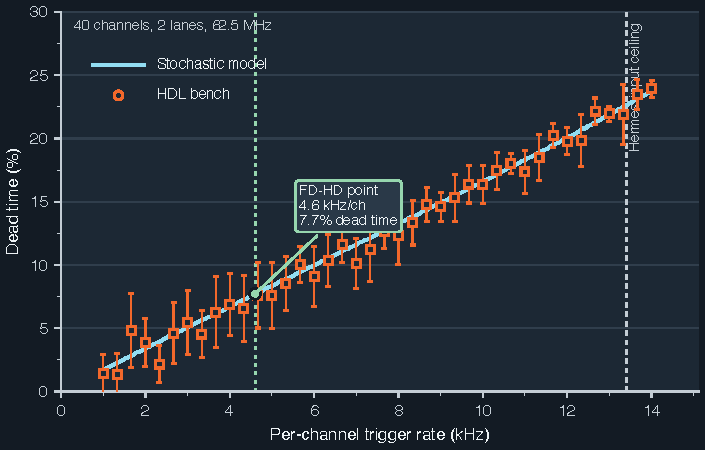
\includegraphics[width=\linewidth,height=0.60\textheight,keepaspectratio]{../daphne_deadtime_apr2026/figures/deadtime_vs_rate_dunenoir_40pt_r8.pdf}
\end{columns}
\end{frame}

\begin{frame}{What The Current Interface Already Covers}
\small
\begin{block}{Already in place}
\begin{itemize}
  \item TP timestamp is waveform timestamp plus sample offset
  \item channel and detector IDs follow \texttt{detchannelmaps}
  \item TP widths, flags, and saturation semantics come from the DAQ TP definition
  \item trailer words survive as extended metadata through \texttt{fddetdataformats}
\end{itemize}
\end{block}

\begin{alertblock}{What still matters on our side}
Validate the DAPHNE-to-TP field content, exercise PDS-oriented TA building, and check rate and loss behavior against board dead-time limits.
\end{alertblock}
\end{frame}

\begin{frame}{Takeaways}
\small
\begin{itemize}
  \item DAPHNE should preserve the \alert{local optical information} that is expensive to recover later: time, width, peak, integral, and quality.
  \item The correct common language downstream is the existing DUNE-DAQ \texttt{TriggerPrimitive} schema.
  \item Detector-scale signatures such as supernova bursts are inherently \alert{multi-board and multi-timescale} problems.
  \item Keep four layers separate: physics signature, firmware descriptor, DAQ trigger object, and detector-level trigger decision.
\end{itemize}
\end{frame}

\begin{frame}{Sources}
\scriptsize
\begin{itemize}
  \item DUNE Collaboration, \emph{ProtoDUNE-DP scintillation light detection}, 2022.
  \item Cattadori for DUNE, \emph{FD1 X-ARAPUCA efficiency and FD2 photon collector upgrade}, 2024.
  \item Brizzolari for DUNE, \emph{Features and performances of the DUNE Far Detector PDS}, 2024/2025.
  \item DUNE Collaboration, \emph{Far Detector Vertical Drift TDR}, 2024.
  \item Andringa et al., \emph{Low-energy physics in neutrino LArTPCs}, 2023.
  \item DUNE-DAQ \texttt{trigger}, \texttt{triggeralgs}, \texttt{detchannelmaps}, and \texttt{fddetdataformats}.
\end{itemize}
\end{frame}

\end{document}
